\chapter{\label{result}Result and Disscusion}

\setcounter{equation}{0}
\setcounter{table}{0}
\setcounter{figure}{0}
% \baselineskip 16pt
\hspace{10pt}\\

\section{$Z\longrightarrow \mu^{+} + \mu^{-}$ process}
\begin{figure}[ht!]
    \centering
    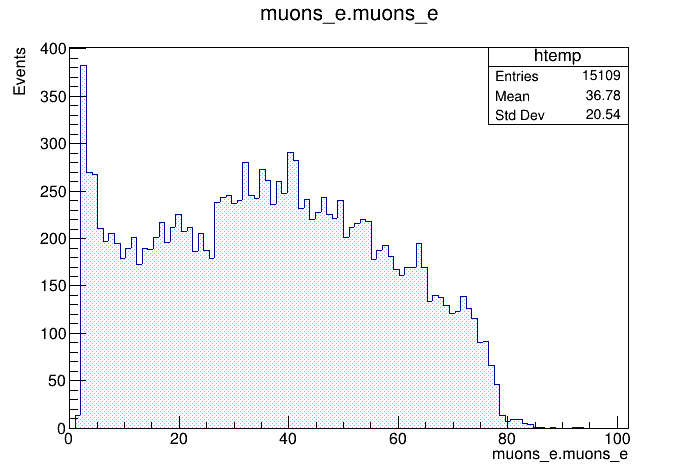
\includegraphics[width=0.5\linewidth]{plots/plots/mue.png}\hfill
    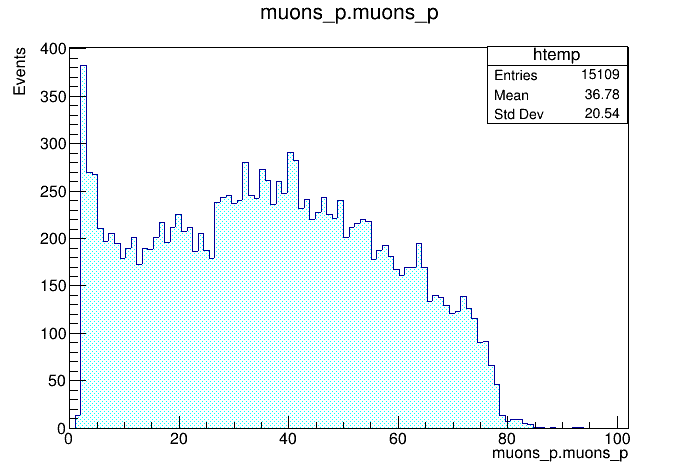
\includegraphics[width=0.5\linewidth]{plots/plots/mup.png}
    \caption{Energy and momentum distribution of $\mu^{+}$ and $\mu^{-}$ at 240GeV.}
\end{figure}

\begin{figure}[ht!]
    \centering
    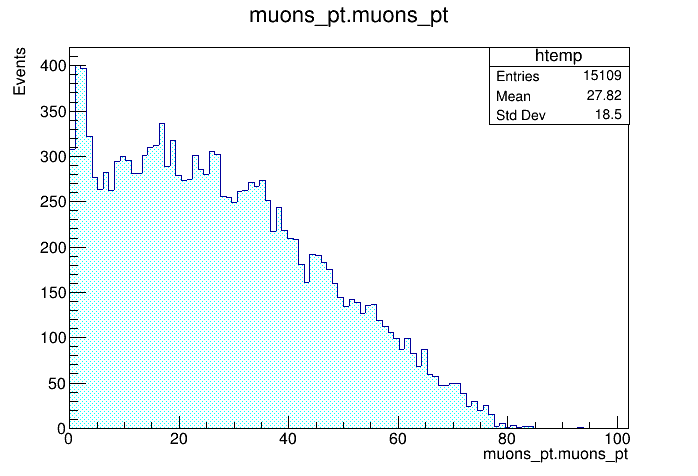
\includegraphics[width=0.5\linewidth]{plots/plots/mupt.png}\hfill
    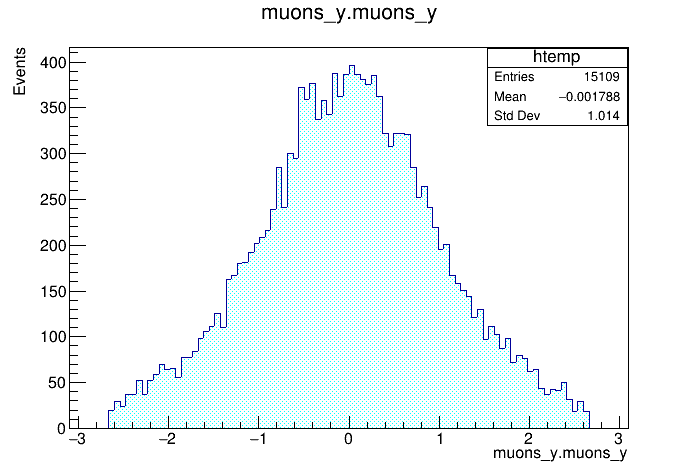
\includegraphics[width=0.5\linewidth]{plots/plots/muy.png}
    \caption{Transverse momentum and rapidity  distribution of $\mu^{+}$ and $\mu^{-}$ at 240GeV.}
\end{figure}

\begin{figure}[ht!]
    \centering
    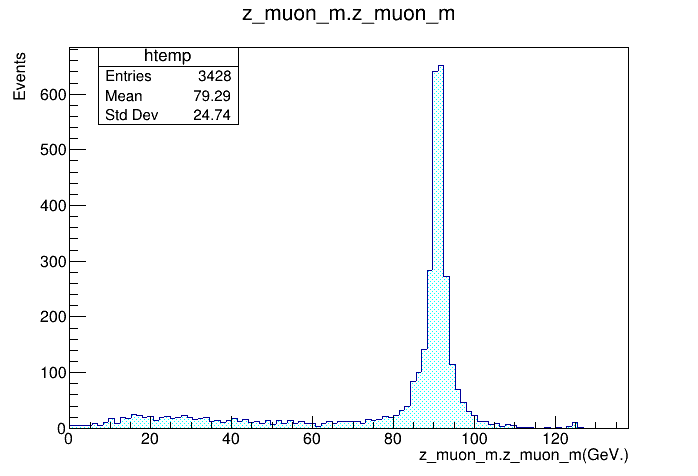
\includegraphics[width=0.5\linewidth]{plots/plots/zmu_m.png}\hfill
    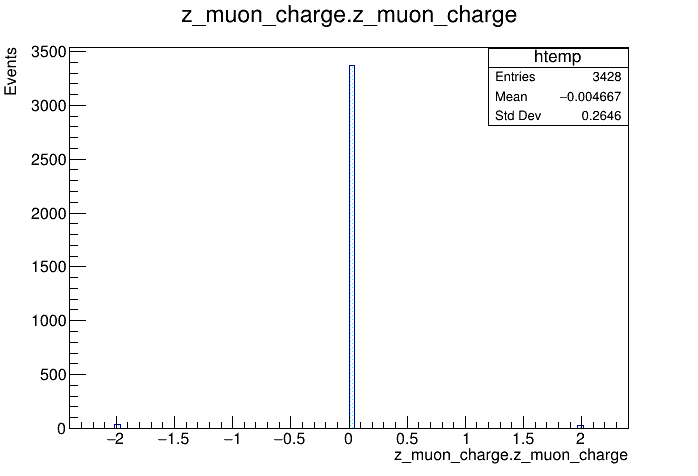
\includegraphics[width=0.5\linewidth]{plots/plots/zmu_charge.png}
    \caption{Reconstructed mass and charge  from  $\mu^{+}$ and $\mu^{-}$ at 240GeV.}
    \label{fig:zmu_mass}
\end{figure}

\begin{figure}[ht!]
    \centering
    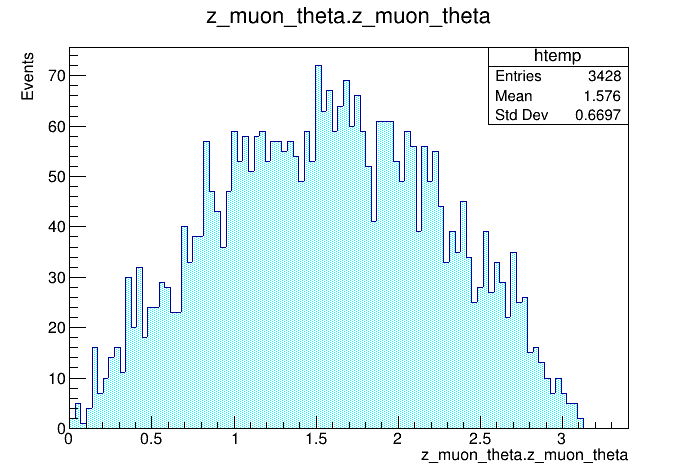
\includegraphics[width=0.5\linewidth]{plots/plots/zmu_theta.png}\hfill
    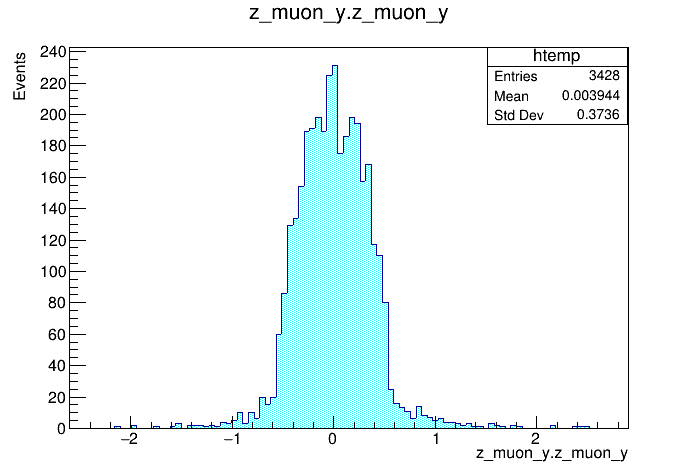
\includegraphics[width=0.5\linewidth]{plots/plots/zmu_y.png}
    \caption{Reconstructed $\theta$ and rapidity  from  $\mu^{+}$ and $\mu^{-}$ at 240GeV.}
\end{figure}

\begin{figure}[ht!]
    \centering
    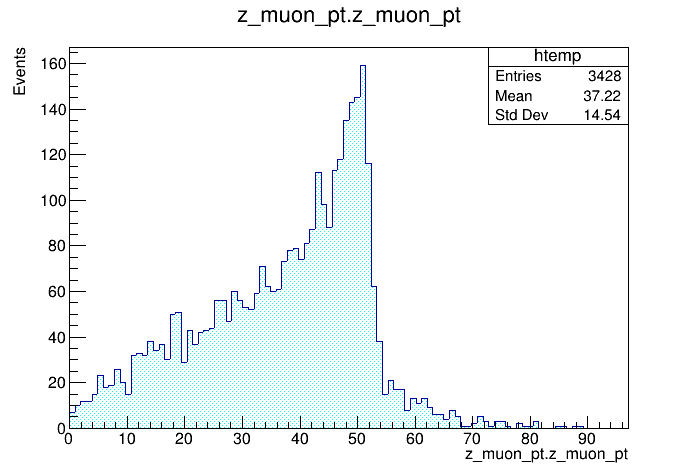
\includegraphics[width=0.5\linewidth]{plots/plots/zmu_pt.png}\hfill
    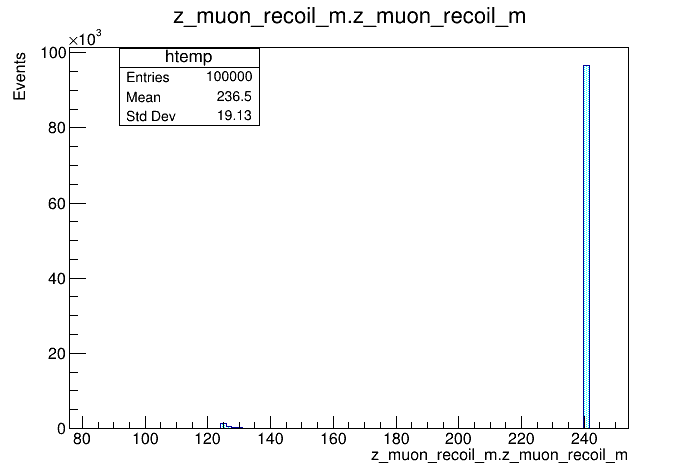
\includegraphics[width=0.5\linewidth]{plots/plots/zmu_recoil_m.png}
    \caption{Reconstructed transverse momentum and recoil mass  from  $\mu^{+}$ and $\mu^{-}$ at 240GeV.}
\end{figure}



\section{$Z\longrightarrow e^{+} + e^{-}$ process}



\begin{figure}[ht!]
    \centering
    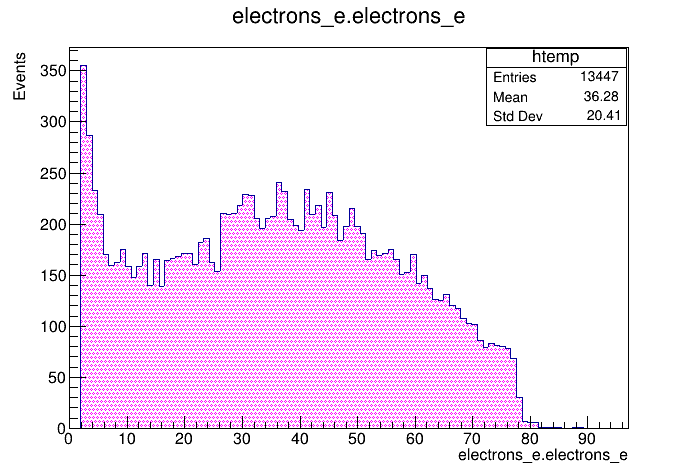
\includegraphics[width=0.5\linewidth]{plots/plots/ee.png}\hfill
    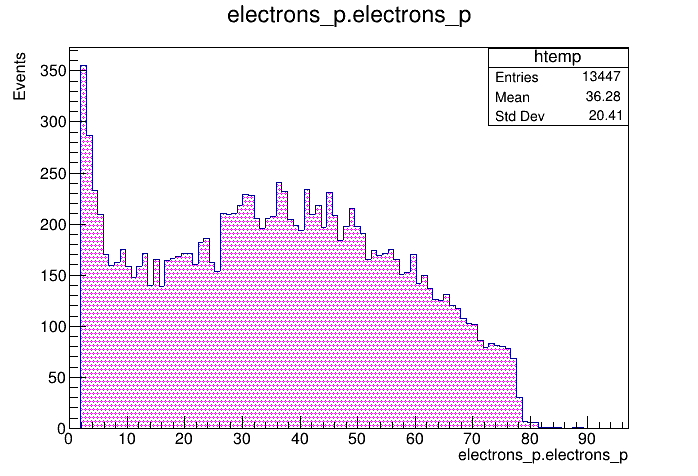
\includegraphics[width=0.5\linewidth]{plots/plots/ep.png}
    \caption{Energy and momentum distribution of $e^{+}$ and $e^{-}$ at 240GeV.}   
\end{figure}

\begin{figure}[ht!]
    \centering
    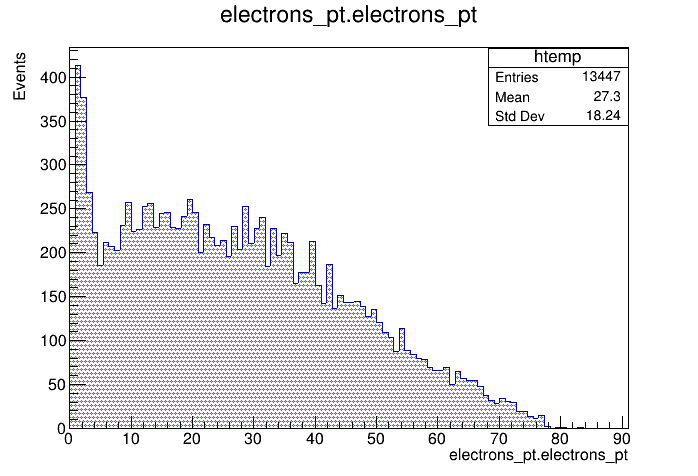
\includegraphics[width=0.5\linewidth]{plots/plots/ept.png}\hfill
    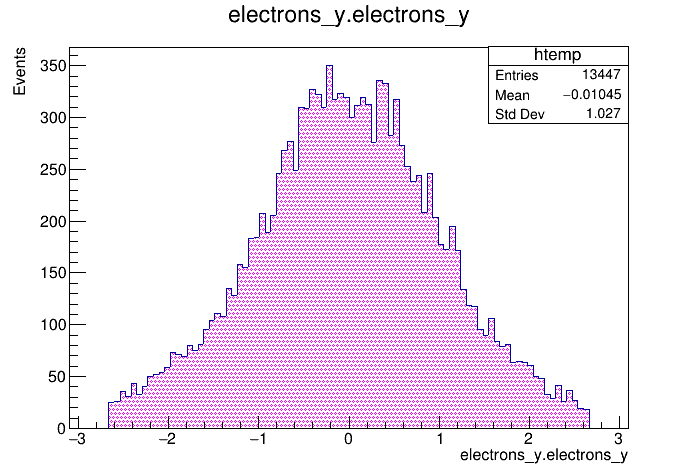
\includegraphics[width=0.5\linewidth]{plots/plots/ey.png}
    \caption{Transverse momentum and rapidity distribution of $e^{+}$ and $e^{-}$ at 240GeV.}                      
\end{figure}


\begin{figure}[ht!]
    \centering
    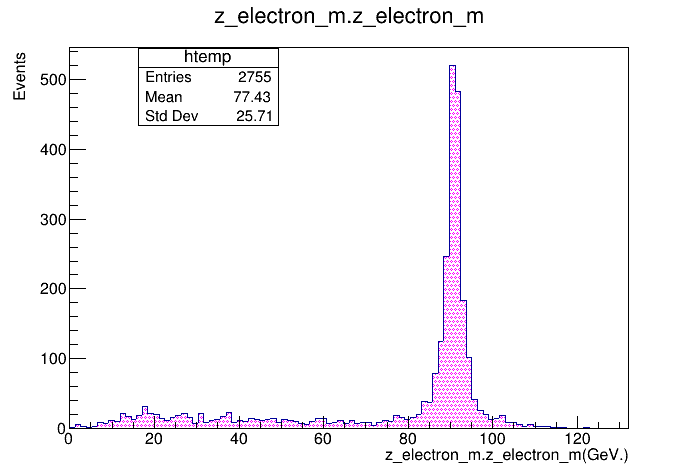
\includegraphics[width=0.5\linewidth]{plots/plots/z_e_m.png}\hfill
    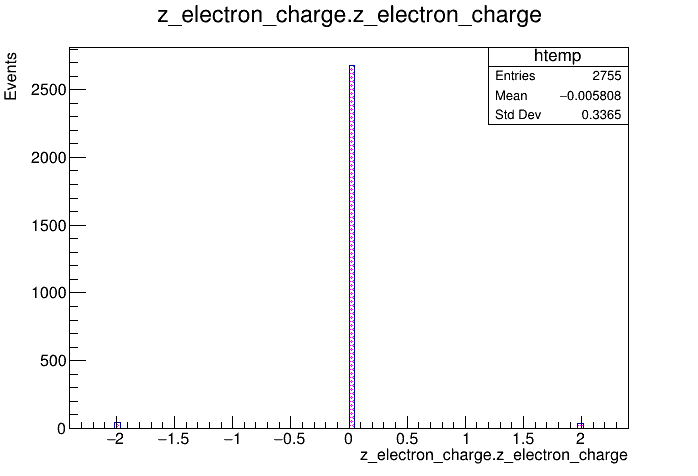
\includegraphics[width=0.5\linewidth]{plots/plots/z_e_charge.png}
    \caption{Reconstructed mass and charge  from  $e^{+}$ and $e^{-}$ at 240GeV.}
    \label{fig:z_e_m}
\end{figure}    
\clearpage

\begin{figure}[ht!]
    \centering
    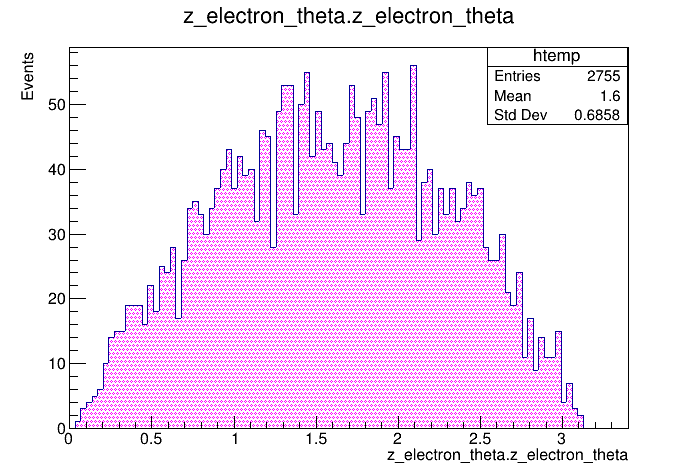
\includegraphics[width=0.5\linewidth]{plots/plots/z_e_theta.png}\hfill
    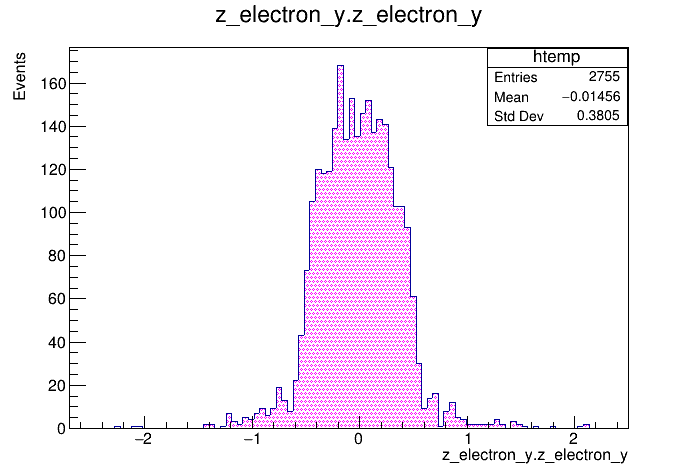
\includegraphics[width=0.5\linewidth]{plots/plots/z_e_y.png}
    \caption{Reconstructed $\theta$ and rapidity  from  $e^{+}$ and $e^{-}$ at 240GeV.}
\end{figure}    

\begin{figure}[ht!]
    \centering
    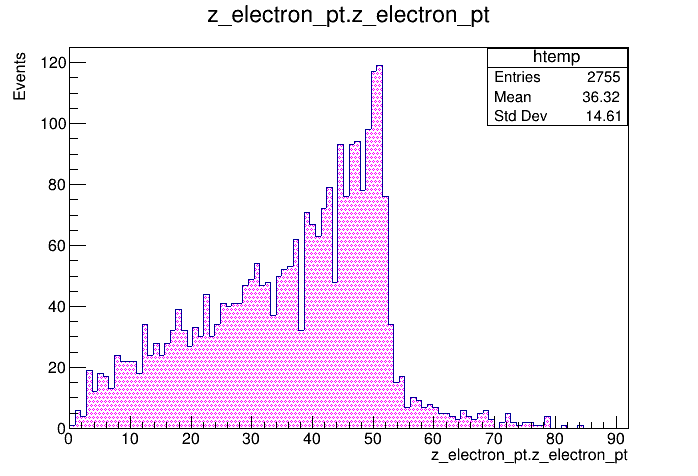
\includegraphics[width=0.5\linewidth]{plots/plots/z_e_pt.png}\hfill
    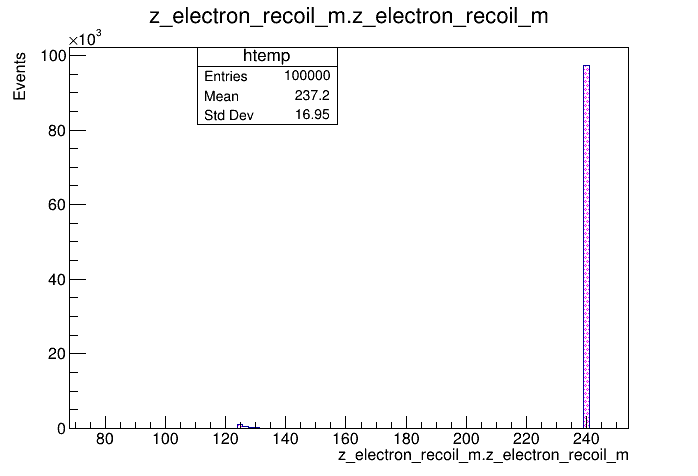
\includegraphics[width=0.5\linewidth]{plots/plots/z_e_recoil_m.png}
    \caption{Reconstructed transverse momentum and recoil mass  from  $e^{+}$ and $e^{-}$ at 240GeV.}
\end{figure}

From figure(\ref{fig:zmu_mass}) and (\ref{fig:z_e_m}) we have got the distributions of the reconstructed Z  mass for $Z\longrightarrow \mu^{+} + \mu^{-}$ and $Z\longrightarrow e^{+} + e^{-}$ respectively.  A peak can be seen around 91GeV. in both distributions, which matches the Z boson mass.

%\section{$H \longrightarrow b + \Bar{b}$ process}
%\section{$e^{+} + e^{-} \longrightarrow H + Z$ process}

%%%%%%%%%%%%%%%%%%%%%%%%%%%%%%%%%%%%%%%%%%%%%%%%%%%%%%%%%%%%%%%%%%%%%%%%%%%%%%